\section{Auswertung}
Die in der Auswertung bestimmten Ausgleichsrechnungen werden mit
dem Python Paket \emph{scipy.optimize}\cite{scipy} durchgeführt.
Des Weiteren werden die Fehler und insbesondere die Fehlerfortpflanzungen
mit dem Python Paket \emph{uncertainties}\cite{uncertainties} berechnet.
Zusätzlich werden die benötigten Naturkonstanten dem Python Paket \emph{scipy.constants}\cite{scipy.constants}
entommen.

\subsection{Untersuchung der Bragg-Bedingung}
Die an der Messapperatur eingestellten Konfiguration lauten:
\begin{equation*}
  \theta=\SI{14}{\degree}, \quad \alpha\ua{GM}\in\left[26,30\right]\,\si{\degree},\quad \Delta\alpha\ua{GM}=\SI{0.1}{\degree}, \quad \Delta t=\SI{10}{\second}.
\end{equation*}
Eine Liste mit den gemessenen Werten ist in Tabelle \ref{} zu finden und in Abbildung \ref{fig: bragg_plot} abgebildet.
\begin{table} 
\centering 
\caption{Messwerte bei der Untersuchung der Bragg Bedingung.} 
\label{tab: bragg_test} 
\begin{tabular}{S S S S } 
\toprule  
{$\alpha_{\mathrm{Gl}} \, / \, \si{\degree}$} & {$I \, / \, \mathrm{Imp}/\mathrm{s}$} & {$\alpha_{\mathrm{Gl}} \, / \, \si{\degree}$} & {$I \, / \, \mathrm{Imp}/\mathrm{s}$}  \\ 
\midrule  
 26.0  & 41  & 28.1  & 156\\ 
26.1  & 41  & 28.2  & 158\\ 
26.2  & 44  & 28.3  & 165\\ 
26.3  & 43  & 28.4  & 168\\ 
26.4  & 47  & 28.5  & 169\\ 
26.5  & 47  & 28.6  & 156\\ 
26.6  & 53  & 28.7  & 148\\ 
26.7  & 56  & 28.8  & 137\\ 
26.8  & 68  & 28.9  & 125\\ 
26.9  & 75  & 29.0  & 119\\ 
27.0  & 73  & 29.1  & 110\\ 
27.1  & 83  & 29.2  & 105\\ 
27.2  & 91  & 29.3  & 91\\ 
27.3  & 102  & 29.4  & 86\\ 
27.4  & 110  & 29.5  & 69\\ 
27.5  & 122  & 29.6  & 66\\ 
27.6  & 118  & 29.7  & 53\\ 
27.7  & 133  & 29.8  & 43\\ 
27.8  & 140  & 29.9  & 40\\ 
27.9  & 150  & 30.0  & 40\\ 
\bottomrule 
\end{tabular} 
\end{table}
\begin{figure}
  \centering
  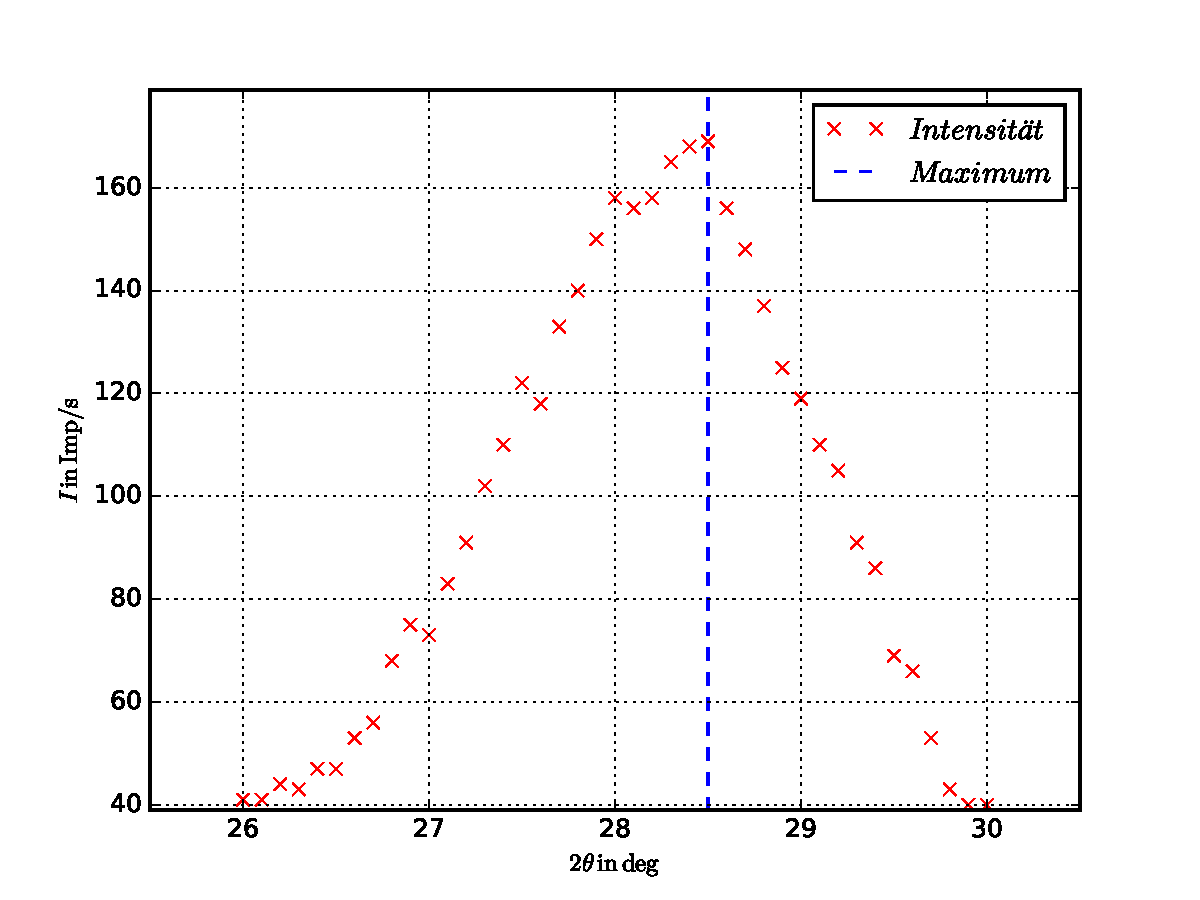
\includegraphics[width=0.8 \textwidth]{../Messdaten/bragbed.pdf}
  \caption{Messwerte zur Untersuchung der Bragg-Bedingung.} %Hingegen passt nicht
  \label{fig: bragg_plot}
\end{figure}
Das Maximum der Messwerte ist der bestimmte Bragg-Winkel:
\begin{equation}
  \label{eq:bestimmt_bragg_winkel}
  2\theta\ua{bragg}=\SI{28.5}{\degree} \quad \Leftrightarrow \quad \theta\ua{bragg}=\SI{14.25}{\degree}.
\end{equation}

\subsection{Untersuchung des Emissionspektrum von $\ce{Cu}$}
Zu Beginn wird der $2:1$ Kopplungsmodus der Apperatur gewählt und folgende Parameter eingestellt:
\begin{equation*}
  \theta\in\left[4,26\right]\,\si{\degree},\quad \Delta\theta\ua{GM}=\SI{0.2}{\degree}, \quad \Delta t=\SI{5}{\second}.
\end{equation*}
Die aufgenommen Werte sind in Tabelle \ref{} aufgelistet und in Abbildung \ref{fig: emission_cu} dargestellt.
\begin{table} 
\centering 
\caption{Messwerte bei der Untersuchung des Emmissionspektrum von $\ce{Cu}$.} 
\label{tab: emi_cu} 
\begin{tabular}{S S } 
\toprule  
{$\theta \, / \, \si{\degree}$} & {$I \, / \, \mathrm{Imp}/\mathrm{s}$}  \\ 
\midrule  
 4.0  & 30.0\\ 
4.2  & 27.0\\ 
4.4  & 29.0\\ 
4.6  & 31.0\\ 
4.8  & 34.0\\ 
5.0  & 43.0\\ 
5.2  & 51.0\\ 
5.4  & 61.0\\ 
5.6  & 64.0\\ 
5.8  & 67.0\\ 
6.0  & 83.0\\ 
6.2  & 87.0\\ 
6.4  & 94.0\\ 
6.6  & 104.0\\ 
6.8  & 118.0\\ 
7.0  & 128.0\\ 
7.2  & 127.0\\ 
7.4  & 145.0\\ 
7.6  & 145.0\\ 
7.8  & 159.0\\ 
8.0  & 156.0\\ 
8.2  & 169.0\\ 
8.3  & 168.0\\ 
8.6  & 178.0\\ 
8.8  & 181.0\\ 
9.0  & 188.0\\ 
9.2  & 185.0\\ 
9.3  & 204.0\\ 
9.6  & 204.0\\ 
9.8  & 198.0\\ 
10.0  & 215.0\\ 
10.2  & 211.0\\ 
10.4  & 225.0\\ 
10.6  & 231.0\\ 
10.8  & 211.0\\ 
11.0  & 235.0\\ 
11.2  & 221.0\\ 
11.4  & 215.0\\ 
11.6  & 218.0\\ 
11.8  & 201.0\\ 
12.0  & 225.0\\ 
12.2  & 220.0\\ 
12.4  & 212.0\\ 
12.6  & 220.0\\ 
12.8  & 195.0\\ 
13.0  & 175.0\\ 
13.2  & 166.0\\ 
13.4  & 176.0\\ 
13.6  & 163.0\\ 
13.8  & 162.0\\ 
14.0  & 163.0\\ 
14.2  & 161.0\\ 
14.4  & 154.0\\ 
14.6  & 153.0\\ 
14.8  & 151.0\\ 
15.0  & 150.0\\ 
15.2  & 145.0\\ 
15.4  & 146.0\\ 
15.6  & 136.0\\ 
15.8  & 137.0\\ 
16.0  & 140.0\\ 
16.2  & 130.0\\ 
16.4  & 130.0\\ 
16.6  & 117.0\\ 
16.8  & 122.0\\ 
17.0  & 126.0\\ 
17.2  & 114.0\\ 
17.4  & 118.0\\ 
17.6  & 105.0\\ 
17.8  & 119.0\\ 
18.0  & 98.0\\ 
18.2  & 110.0\\ 
18.4  & 104.0\\ 
18.6  & 112.0\\ 
18.8  & 119.0\\ 
19.0  & 101.0\\ 
19.2  & 110.0\\ 
19.4  & 121.0\\ 
19.6  & 464.0\\ 
19.8  & 1194.0\\ 
20.0  & 761.0\\ 
20.2  & 169.0\\ 
20.4  & 147.0\\ 
20.6  & 123.0\\ 
20.8  & 120.0\\ 
21.0  & 116.0\\ 
21.2  & 113.0\\ 
21.4  & 122.0\\ 
21.6  & 165.0\\ 
21.8  & 316.0\\ 
22.0  & 4140.0\\ 
22.2  & 3604.0\\ 
22.4  & 333.0\\ 
22.6  & 144.0\\ 
22.8  & 110.0\\ 
23.0  & 92.0\\ 
23.2  & 86.0\\ 
23.4  & 83.0\\ 
23.6  & 67.0\\ 
23.8  & 75.0\\ 
24.0  & 69.0\\ 
24.2  & 67.0\\ 
24.4  & 64.0\\ 
24.6  & 61.0\\ 
24.8  & 60.0\\ 
25.0  & 58.0\\ 
25.2  & 0.0\\ 
25.4  & 54.0\\ 
25.6  & 55.0\\ 
25.8  & 48.0\\ 
26.0  & 45.0\\ 
\bottomrule 
\end{tabular} 
\end{table}
\begin{figure}
  \centering
  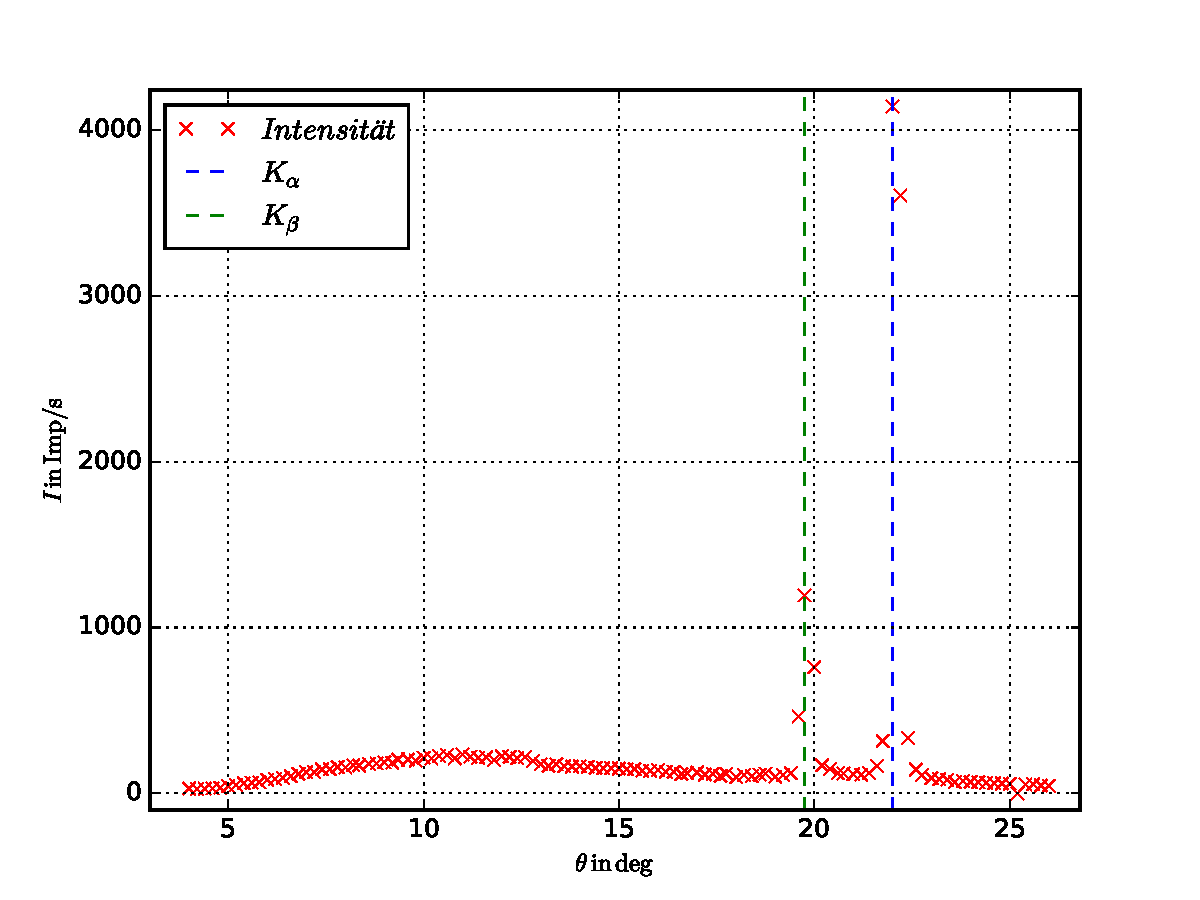
\includegraphics[width=0.8 \textwidth]{../Messdaten/emission_cu.pdf}
  \caption{Messsung des Emmissionspektrums von $\ce{Cu}$.} %Hingegen passt nicht
  \label{fig: emission_cu}
\end{figure}
In der Abbildung sind die $K_\alpha$ und $K_\beta$ Kante mit eingezeichnet.
Aus dem Experiment ergebens sich die folgenden Werte:
\begin{equation}
  \label{eq:k_alpha,k_beta}
  K_\alpha=\SI{8.2}{\kilo\eV} \qquad   K_\beta=\SI{9.1}{\kilo\eV}.
\end{equation}
Die maximale Energie beläuft sich auf:
\begin{equation}
  \label{eq: maximale_energie}
  E\ua{max}=\SI{44.1}{\kilo\eV}
\end{equation}
Die Winkel werden dabei mit Gleichung \eqref{} umgerechnet.
Mit Hilfe der Energien \eqref{eq:k_alpha,k_beta}, können die Abschirmkonstanten
für die einzelnen K- Linien bestimmt werden.
Aus den Formeln \eqref{} errechnet sich:
\begin{equation}
   \label{eq:abschirm}
   \sigma_1=3.13 \qquad \simga_2=20.9.
\end{equation}

\textbf{Es fehlt noch die Halbwertsbreite}
